% Auto-generated from Markdown by scripts/generateLatexDocumentation.js
% Compile with XeLaTeX or LuaLaTeX for Bangla/English Unicode support.
\documentclass[12pt,a4paper]{report}
\usepackage[a4paper,margin=1in]{geometry}
\usepackage{fontspec}
\IfFontExistsTF{Nirmala UI}{\setmainfont{Nirmala UI}}{\setmainfont{FreeSerif}}
\IfFontExistsTF{Consolas}{\setmonofont{Consolas}}{\setmonofont{DejaVu Sans Mono}}
\usepackage{graphicx}
\usepackage{xcolor}
\usepackage{hyperref}
\usepackage{longtable}
\usepackage{array}
\usepackage{enumitem}
\usepackage{fancyhdr}
\usepackage{fvextra}
\usepackage{caption}
\hypersetup{colorlinks=true,linkcolor=blue,urlcolor=blue}
\DefineVerbatimEnvironment{CodeBlock}{Verbatim}{breaklines,breakanywhere,fontsize=\small}
\setlist[itemize]{topsep=4pt,itemsep=2pt,parsep=0pt}
\setlist[enumerate]{topsep=4pt,itemsep=2pt,parsep=0pt}
\pagestyle{fancy}
\fancyhf{}
\lhead{Amiyo-Go}
\rhead{Documentation}
\cfoot{\thepage}
\title{Amiyo-Go Marketplace Thesis Documentation}
\author{Amiyo-Go Engineering}
\date{Generated 2026-06-04 from AMIYO\_GO\_THESIS\_DOCUMENTATION.md}
\begin{document}
\maketitle
\tableofcontents
\clearpage

\chapter{Amiyo-Go Marketplace Thesis Documentation}

\textbf{Project:} Amiyo-Go Multi-Vendor Marketplace

\textbf{Document type:} Thesis-style technical documentation

\textbf{Last updated:} 2026-06-04

\textbf{Prepared for:} Product, engineering, operations, vendor, and admin review


\begin{CodeBlock}
---
\end{CodeBlock}

\section{Abstract}

Amiyo-Go is a role-based multi-vendor marketplace system designed to support customer shopping, vendor seller-center operations, and admin marketplace governance. The project has evolved beyond a simple ecommerce catalog into a marketplace operating system with modules for catalog management, vendor onboarding, order fulfillment, courier workflow, returns, payments, promotions, trust and safety, analytics, staff permissions, and documentation/training.


The application follows a modular monolith architecture. The frontend is built with React, React Router, Tailwind CSS, reusable UI components, and role-specific layouts. The backend is a Node.js and Express API layer using MongoDB through Mongoose and native MongoDB access. Selected background workflows use BullMQ/Redis where configured. The system includes adapter-ready integrations for courier providers, payment providers, notification channels, object storage, and search provider abstraction.


This documentation records the full implementation scope, current architecture, feature inventory, role workflows, data model map, API surface, quality practices, deployment notes, known limitations, and future production-hardening roadmap. It is intended to work as a project thesis, handover document, and production-readiness reference.


\section{Keywords}

Marketplace, ecommerce, multi-vendor, seller center, admin dashboard, logistics, COD, returns, trust and safety, analytics, promotions, React, Node.js, Express, MongoDB, Firebase, BullMQ.


\begin{CodeBlock}
---
\end{CodeBlock}

\section{Table of Contents}

\begin{enumerate}
\item Introduction
\item Project Goals and Scope
\item Stakeholder and Role Analysis
\item Technology Stack
\item System Architecture and UI Screenshots
\item Frontend Architecture
\item Backend Architecture
\item Database and Persistence Model
\item Feature Documentation by Role
\item Business Workflows
\item API and Service Map
\item Security, Trust, and Permissions
\item Logistics and Courier Integration
\item Promotions, Growth, and Personalization
\item Analytics and Reporting
\item Testing and Quality Assurance
\item Deployment and Environment Configuration
\item Documentation and Training Layer
\item Production-Readiness Assessment
\item Limitations and Future Work
\item Conclusion
\item Appendices
\end{enumerate}

\begin{CodeBlock}
---
\end{CodeBlock}

\chapter{Chapter 1: Introduction}

\section{1.1 Background}

Modern marketplaces are not only product listing websites. They are operational platforms where customers, sellers, and platform operators coordinate through structured workflows. A Daraz-level marketplace needs customer discovery and checkout, seller-center controls, logistics state tracking, finance settlement, dispute handling, campaign tools, analytics, and staff governance.


Amiyo-Go is designed around that concept. The project connects customer shopping actions, vendor operating tools, and admin governance into one system. The core value is not only that products can be purchased, but that the marketplace can be managed after the order is placed.


\section{1.2 Problem Statement}

A normal ecommerce application usually solves only these problems:


\begin{itemize}
\item Display products.
\item Add products to cart.
\item Place an order.
\item Let an admin view orders.
\end{itemize}

A real marketplace must solve many more:


\begin{itemize}
\item Sellers need onboarding, KYC, product moderation, stock management, packing, finance, promotions, and reputation tools.
\item Customers need trustworthy shopping, order tracking, invoices, returns, refunds, support, reviews, saved addresses, alerts, loyalty, and notifications.
\item Admins need vendor approval, moderation queues, dispatch controls, COD reconciliation, payment verification, payout management, trust and safety, analytics, staff permissions, and audit logs.
\item Operators need clear documentation and training so each role understands what they should see and do.
\end{itemize}

Amiyo-Go addresses these needs through a modular marketplace workflow.


\section{1.3 Project Aim}

The aim of Amiyo-Go is to provide a production-oriented marketplace foundation that can operate with manual workflows first and gradually attach paid/external integrations such as courier APIs, payment gateways, SMS providers, object storage, and search engines.


\section{1.4 Thesis Objective}

This document has four objectives:


\begin{enumerate}
\item Explain the complete project architecture.
\item Document all major customer, vendor, and admin features.
\item Record operational workflows and implementation status.
\item Provide a production-readiness reference for future hardening.
\end{enumerate}

\begin{CodeBlock}
---
\end{CodeBlock}

\chapter{Chapter 2: Project Goals and Scope}

\section{2.1 Functional Goals}

The main functional goals are:


\begin{itemize}
\item Build a three-role marketplace: customer, vendor, and admin.
\item Allow customers to browse, search, purchase, track, return, review, and get support.
\item Allow vendors to manage shop, KYC, catalog, inventory, orders, fulfillment, returns, finance, marketing, Q\&A, reviews, and reports.
\item Allow admins to manage vendors, products, orders, returns, payouts, COD, logistics, promotions, trust, staff, analytics, and platform settings.
\item Support customer-facing shop storefronts with follow/unfollow and vendor products.
\item Support marketplace growth through promotions, flash sales, loyalty, recommendations, alerts, and notifications.
\item Support logistics through internal shipment state machines and adapter-ready courier booking.
\item Support role learning through Amiyo-Go University with protected vendor/admin learning content.
\end{itemize}

\section{2.2 Non-Functional Goals}

Important non-functional goals include:


\begin{itemize}
\item Maintainable modular monolith design.
\item Role-based access control.
\item Secure API boundaries.
\item Responsive frontend UI.
\item Progressive Web App readiness.
\item Auditable admin and finance actions.
\item Extensible integration adapters.
\item Documentation-first handover.
\item Testable frontend and backend modules.
\end{itemize}

\section{2.3 Scope Boundary}

The project currently includes many production-grade foundations, but some external systems remain environment-dependent:


\begin{itemize}
\item MongoDB is the current database. PostgreSQL is not the current implementation.
\item Redis and BullMQ exist for selected background workflows, but they are not yet universal for every event.
\item Courier APIs are adapter-ready. Manual and internal courier workflows remain valid without paid courier API activation.
\item Payment provider adapters exist, but production payment depth depends on provider credentials and webhook configuration.
\item Email, push, and optional SMS rely on configured providers.
\item Object storage/upload provider behavior depends on environment configuration.
\end{itemize}

\begin{CodeBlock}
---
\end{CodeBlock}

\chapter{Chapter 3: Stakeholder and Role Analysis}

\section{3.1 Customer}

The customer is the buyer role. Customers use the marketplace to discover products, compare options, place orders, track delivery, request returns, review products, and contact support.


Customer priorities:


\begin{itemize}
\item Trustworthy product information.
\item Clear prices and discounts.
\item Smooth checkout.
\item Accurate order tracking.
\item Easy returns and support.
\item Useful recommendations and alerts.
\end{itemize}

\section{3.2 Vendor}

The vendor is the seller role. Vendors use Amiyo-Go as a seller center to manage shop identity, products, stock, orders, packing, dispatch, returns, finance, promotions, reviews, and support communication.


Vendor priorities:


\begin{itemize}
\item Clear onboarding and KYC status.
\item Product approval workflow.
\item Fast order handling.
\item Finance clarity.
\item Campaign and voucher tools.
\item Shop reputation and customer communication.
\end{itemize}

\section{3.3 Admin}

The admin is the marketplace operator role. Admins control the platform through queues, policies, settings, staff permissions, audit logs, moderation, logistics, finance, trust, and analytics.


Admin priorities:


\begin{itemize}
\item Central visibility.
\item Exception handling.
\item Approval workflows.
\item Fraud and dispute control.
\item Revenue and payout accuracy.
\item Staff access governance.
\item Operational dashboards.
\end{itemize}

\begin{CodeBlock}
---
\end{CodeBlock}

\chapter{Chapter 4: Technology Stack}

\section{4.1 Frontend Stack}

\begin{CodeBlock}
| Area | Technology |
\end{CodeBlock}
\begin{CodeBlock}
| --- | --- |
\end{CodeBlock}
\begin{CodeBlock}
| Framework | React |
\end{CodeBlock}
\begin{CodeBlock}
| Router | React Router |
\end{CodeBlock}
\begin{CodeBlock}
| Build tool | Vite |
\end{CodeBlock}
\begin{CodeBlock}
| Styling | Tailwind CSS and reusable UI components |
\end{CodeBlock}
\begin{CodeBlock}
| Icons | lucide-react |
\end{CodeBlock}
\begin{CodeBlock}
| HTTP | axios and fetch patterns |
\end{CodeBlock}
\begin{CodeBlock}
| Forms | react-hook-form where used |
\end{CodeBlock}
\begin{CodeBlock}
| Charts | Chart.js, Recharts |
\end{CodeBlock}
\begin{CodeBlock}
| Maps | Leaflet and react-leaflet |
\end{CodeBlock}
\begin{CodeBlock}
| Notifications | react-hot-toast, push subscription UI |
\end{CodeBlock}
\begin{CodeBlock}
| i18n | i18next and react-i18next |
\end{CodeBlock}
\begin{CodeBlock}
| PWA | Manifest and service worker support |
\end{CodeBlock}
\begin{CodeBlock}
| Tests | Jest, React Testing Library |
\end{CodeBlock}

\section{4.2 Backend Stack}

\begin{CodeBlock}
| Area | Technology |
\end{CodeBlock}
\begin{CodeBlock}
| --- | --- |
\end{CodeBlock}
\begin{CodeBlock}
| Runtime | Node.js |
\end{CodeBlock}
\begin{CodeBlock}
| API framework | Express |
\end{CodeBlock}
\begin{CodeBlock}
| Database | MongoDB |
\end{CodeBlock}
\begin{CodeBlock}
| ODM | Mongoose |
\end{CodeBlock}
\begin{CodeBlock}
| Native database access | mongodb package where needed |
\end{CodeBlock}
\begin{CodeBlock}
| Auth integration | Firebase Admin SDK |
\end{CodeBlock}
\begin{CodeBlock}
| File upload | multer, upload service, storage adapters |
\end{CodeBlock}
\begin{CodeBlock}
| PDF generation | pdfkit |
\end{CodeBlock}
\begin{CodeBlock}
| Queues | BullMQ and Redis where configured |
\end{CodeBlock}
\begin{CodeBlock}
| Email | nodemailer and email services |
\end{CodeBlock}
\begin{CodeBlock}
| Push | web-push |
\end{CodeBlock}
\begin{CodeBlock}
| Payments | Provider adapter services including bKash/Nagad/SSLCommerz/Stripe patterns |
\end{CodeBlock}
\begin{CodeBlock}
| Courier | Courier provider service and Amiyo Delivery integration service |
\end{CodeBlock}
\begin{CodeBlock}
| Security | helmet, cors, rate limit, sanitization |
\end{CodeBlock}
\begin{CodeBlock}
| Logging | winston |
\end{CodeBlock}
\begin{CodeBlock}
| Tests | Jest, Supertest |
\end{CodeBlock}

\section{4.3 Infrastructure and Integrations}

External or optional integrations include:


\begin{itemize}
\item Firebase authentication and admin claims.
\item MongoDB Atlas or local MongoDB.
\item Redis for queues where enabled.
\item Email provider.
\item Web push provider keys.
\item Courier providers such as RedX, Steadfast, local/internal delivery, and Amiyo Delivery integration.
\item Payment gateways and manual payment verification.
\item Object storage adapters.
\end{itemize}

\begin{CodeBlock}
---
\end{CodeBlock}

\chapter{Chapter 5: System Architecture}

\section{5.1 Architectural Style}

Amiyo-Go uses a modular monolith architecture. All business domains are inside one backend application, but each major domain has its own routes, controllers, models, services, utilities, and frontend pages.


This architecture is appropriate because:


\begin{itemize}
\item It is easier to develop and test than microservices.
\item It keeps cross-domain workflows in one codebase.
\item It allows future extraction of heavy modules if scale demands it.
\item It supports fast iteration for marketplace features.
\end{itemize}

\section{5.2 High-Level System Flow}

\begin{CodeBlock}
Customer Web App / Vendor Dashboard / Admin Dashboard
-> React frontend with role-based layouts and guards
-> Express API
-> Domain route modules
-> Services and utilities
-> MongoDB collections/models
-> Optional queues, storage, courier, payment, email, push
\end{CodeBlock}

\section{5.3 Main Backend Domains}

The backend registers route groups for:


\begin{itemize}
\item Products and catalog.
\item Search and discovery.
\item Categories and dynamic categories.
\item Orders and vendor orders.
\item Shipments and logistics.
\item Users, accounts, addresses.
\item Wishlist and alerts.
\item Reviews and Q\&A.
\item Coupons, vouchers, offers, campaigns, promotions.
\item Returns and refunds.
\item Payments and webhooks.
\item Support and chats.
\item Flash sales and recommendations.
\item Growth systems.
\item Trust and safety.
\item Platform settings.
\item Delivery settings and courier rules.
\item Vendor staff, KYC, shop, products, logistics, finance, growth.
\item Admin users, vendors, products, payments, banners, settings, staff, COD, reviews, finance, payouts, analytics, logistics, customers, platform, audit.
\end{itemize}

\section{5.4 Frontend Role Layouts}

The frontend separates role experience through:


\begin{itemize}
\item Main/customer layout.
\item Vendor layout.
\item Admin layout.
\item Route guards.
\item Role-specific navigation.
\item Protected University pages for vendor/admin training.
\end{itemize}

\section{5.5 Screenshot Walkthrough and How It Works}

This screenshot set was captured from the running frontend on 2026-06-04. It intentionally uses public and access pages only, so the PDF does not expose private admin/vendor data or real customer records. Protected vendor/admin dashboards are documented through workflows and route descriptions instead of unauthenticated screenshots.


এই স্ক্রিনশটগুলো ২০২৬-০৬-০৪ তারিখে রানিং frontend থেকে নেওয়া হয়েছে। এখানে শুধু public/access page ব্যবহার করা হয়েছে, তাই PDF-এ private admin/vendor data বা real customer record প্রকাশ করা হয়নি। Protected vendor/admin dashboard স্ক্রিনশটের বদলে workflow এবং route description দিয়ে ব্যাখ্যা করা হয়েছে।


\subsection{Figure 1: Customer Home Page}

\begin{figure}[htbp]
\centering
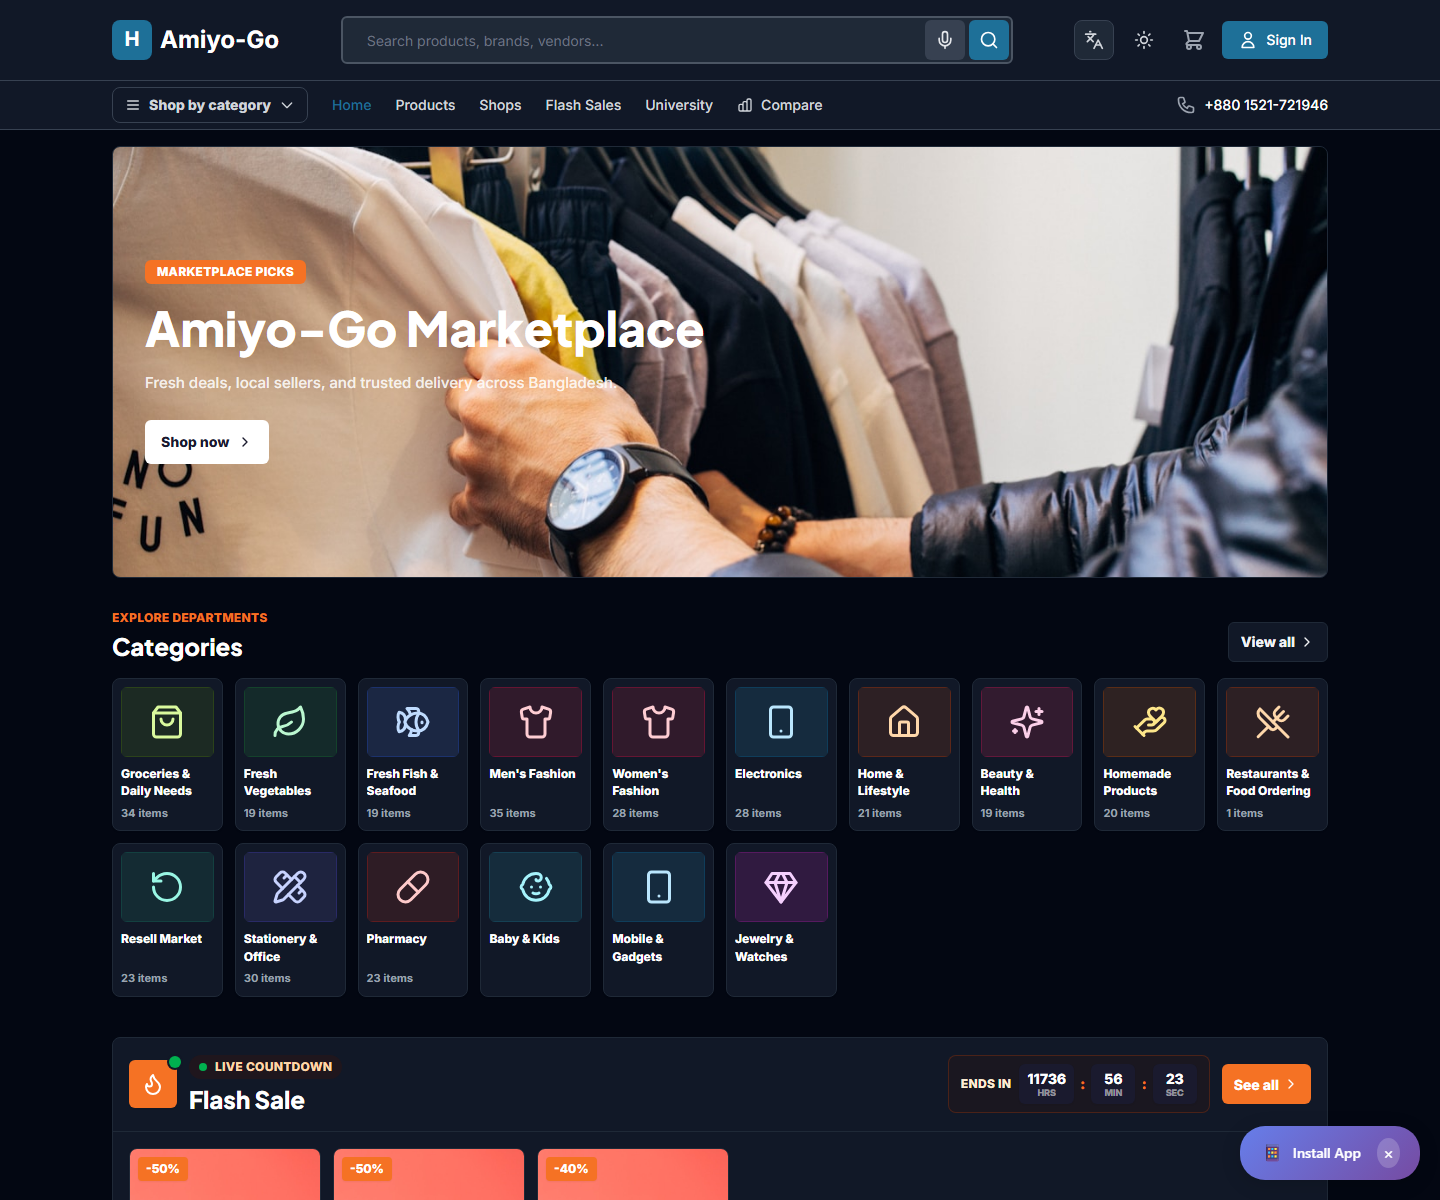
\includegraphics[width=\linewidth,height=0.58\textheight,keepaspectratio]{docs/thesis-screenshots/01-home-desktop.png}
\caption{Customer home page with modern marketplace sections}
\end{figure}


\textbf{How it works in English:}


\begin{itemize}
\item The customer enters through the home page.
\item The header gives search, category navigation, product links, shops, flash sales, compare, language, theme, cart, and sign-in access.
\item The hero area promotes the marketplace and sends users into shopping.
\item Category, flash sale, product, and shop sections help users discover products quickly.
\item Admin-controlled banners and sections can change the front page without code changes.
\end{itemize}

\textbf{কীভাবে কাজ করে বাংলায়:}


\begin{itemize}
\item কাস্টমার home page দিয়ে marketplace-এ প্রবেশ করে।
\item Header থেকে search, category, product, shops, flash sale, compare, language, theme, cart এবং sign-in access পাওয়া যায়।
\item Hero section marketplace offer দেখায় এবং user-কে shopping flow-তে নিয়ে যায়।
\item Category, flash sale, product এবং shop section দ্রুত product discovery করতে সাহায্য করে।
\item Admin-controlled banner এবং section code change ছাড়াই homepage update করতে পারে।
\end{itemize}

\subsection{Figure 2: Customer Learning Center}

\begin{figure}[htbp]
\centering
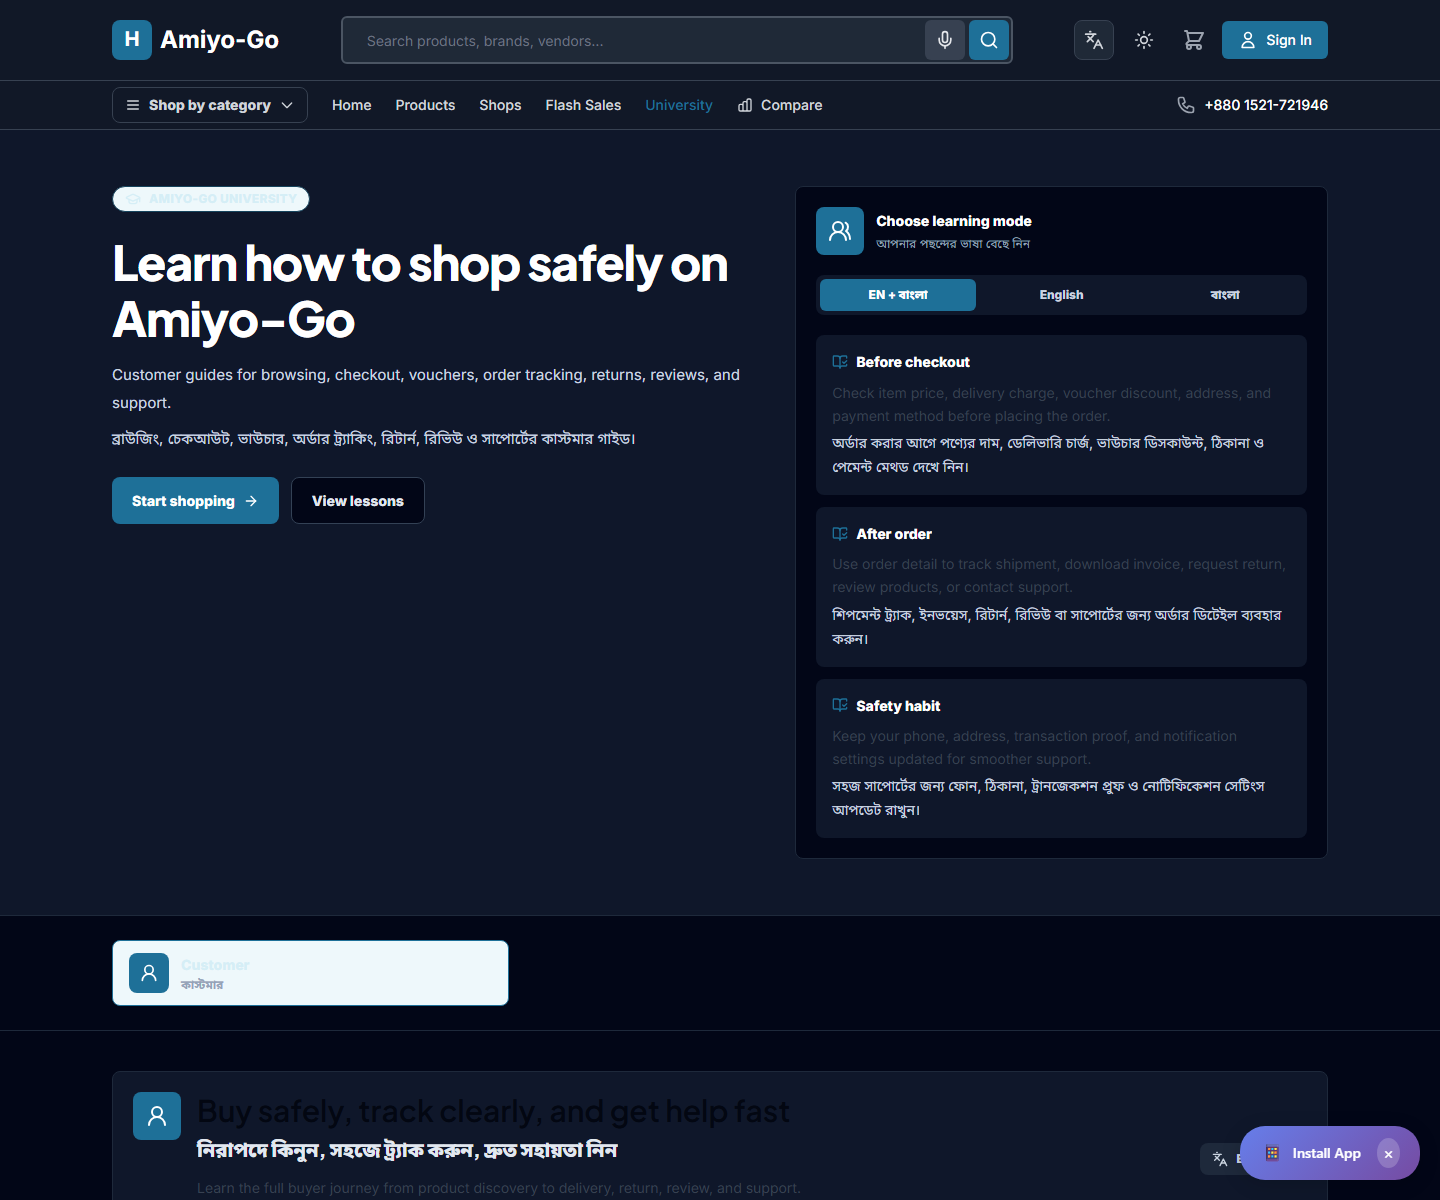
\includegraphics[width=\linewidth,height=0.58\textheight,keepaspectratio]{docs/thesis-screenshots/02-customer-university.png}
\caption{Customer-only Amiyo-Go University page}
\end{figure}


\textbf{How it works in English:}


\begin{itemize}
\item Public users only see customer learning content on \texttt{/university}.
\item Vendor and admin operating lessons are not bundled into the public route.
\item Customers learn checkout, vouchers, order tracking, returns, reviews, and support.
\item Language mode supports English, Bangla, or both together.
\end{itemize}

\textbf{কীভাবে কাজ করে বাংলায়:}


\begin{itemize}
\item Public user \texttt{/university} পেজে শুধু customer guide দেখে।
\item Vendor/admin operating lesson public route-এ bundle করা হয় না।
\item Customer checkout, voucher, order tracking, return, review এবং support শেখে।
\item Language mode English, Bangla বা দুই ভাষা একসাথে support করে।
\end{itemize}

\subsection{Figure 3: Shop Discovery}

\begin{figure}[htbp]
\centering
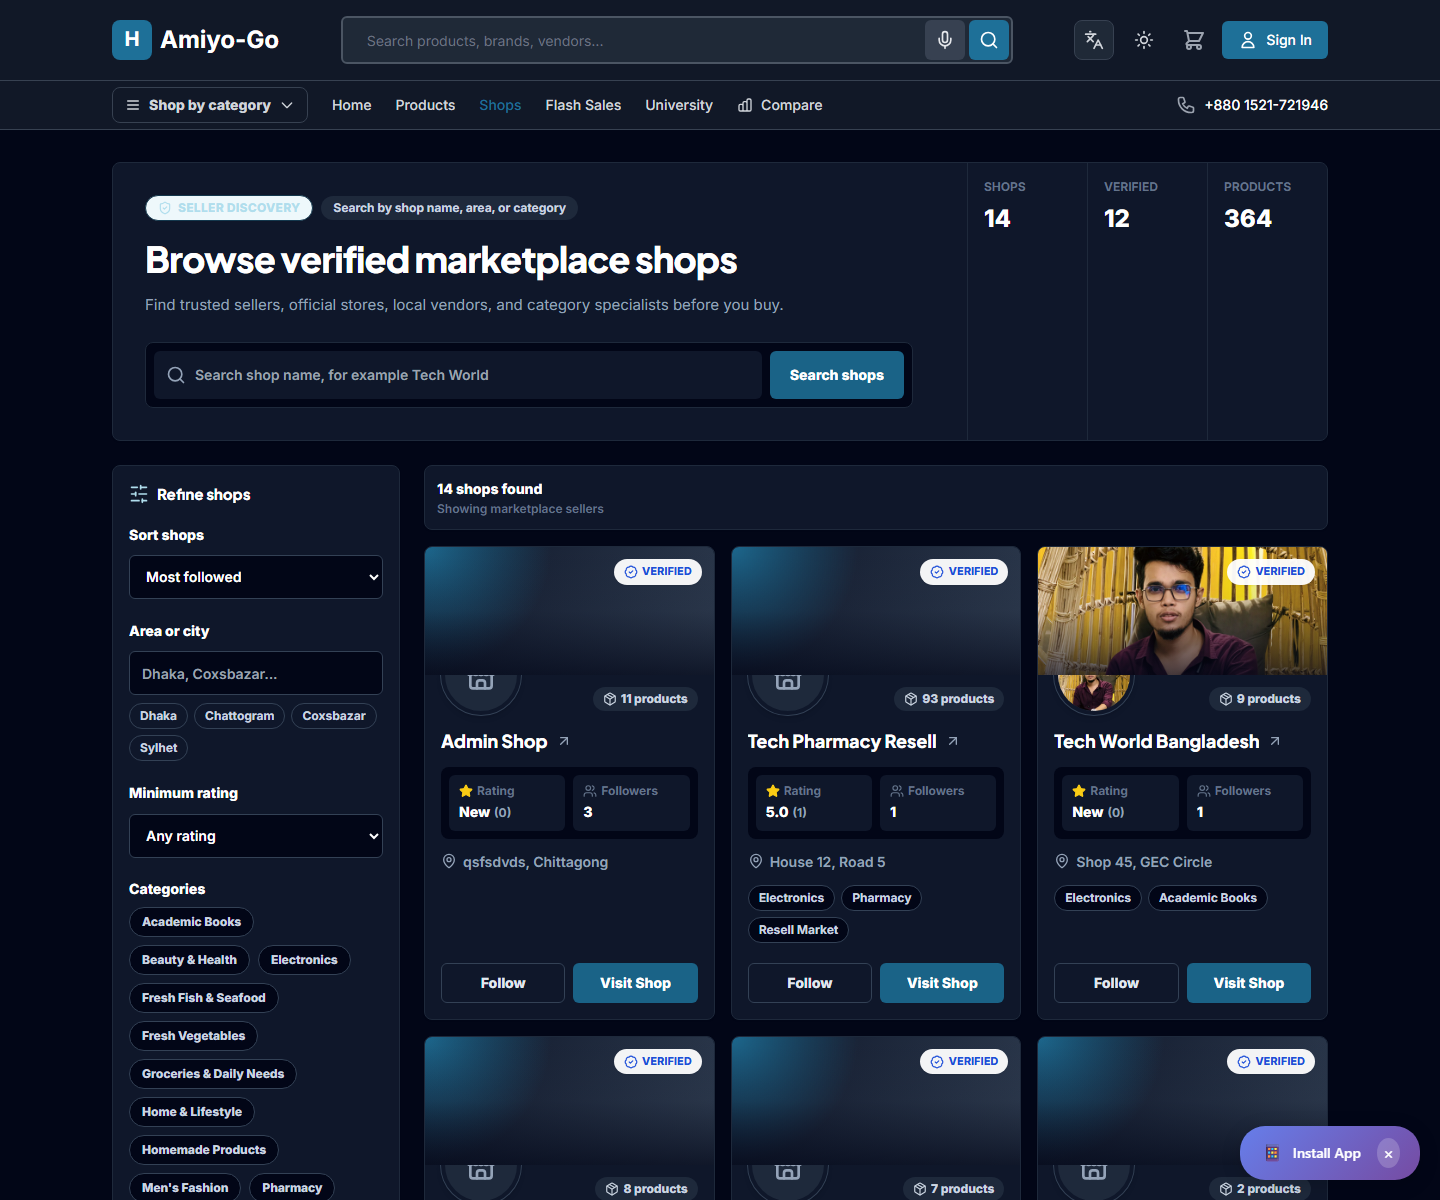
\includegraphics[width=\linewidth,height=0.58\textheight,keepaspectratio]{docs/thesis-screenshots/03-shops-discovery.png}
\caption{Shop discovery page with filters, shop cards, and follow action}
\end{figure}


\textbf{How it works in English:}


\begin{itemize}
\item Customers can browse verified marketplace shops.
\item Search supports shop name, area, and category intent.
\item Filters allow sorting by popularity, location, rating, and category.
\item Each shop card shows trust signals, product count, follower count, location, and visit/follow actions.
\item The backend \texttt{/api/shops} route returns safe public vendor fields only.
\end{itemize}

\textbf{কীভাবে কাজ করে বাংলায়:}


\begin{itemize}
\item Customer verified marketplace shop browse করতে পারে।
\item Search shop name, area এবং category intent support করে।
\item Filter দিয়ে popularity, location, rating এবং category অনুযায়ী result দেখা যায়।
\item Shop card-এ trust signal, product count, follower count, location, visit এবং follow action থাকে।
\item Backend \texttt{/api/shops} route শুধু safe public vendor field return করে।
\end{itemize}

\subsection{Figure 4: Account Registration and Address Capture}

\begin{figure}[htbp]
\centering
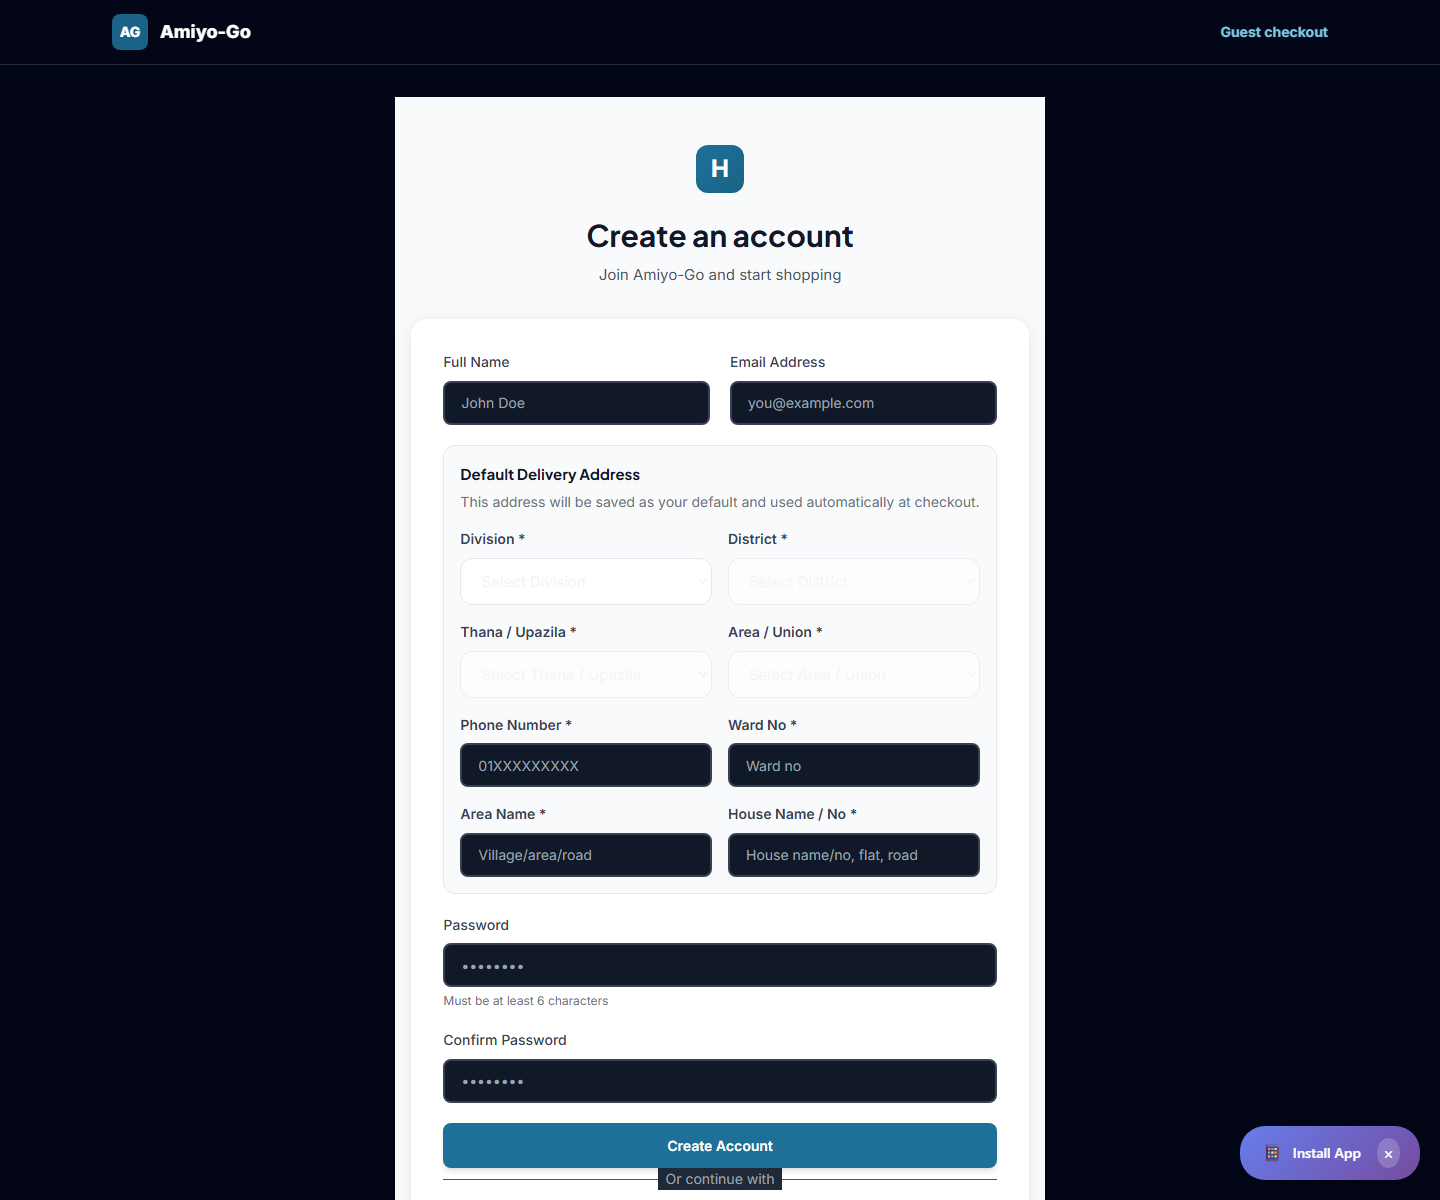
\includegraphics[width=\linewidth,height=0.58\textheight,keepaspectratio]{docs/thesis-screenshots/04-account-registration.png}
\caption{Customer registration page with default address fields}
\end{figure}


\textbf{How it works in English:}


\begin{itemize}
\item A new customer creates an account before using full account features.
\item Registration captures basic identity and default delivery address.
\item Address fields are structured for Bangladesh delivery workflow.
\item The saved address later supports checkout, delivery calculation, courier assignment, and support.
\end{itemize}

\textbf{কীভাবে কাজ করে বাংলায়:}


\begin{itemize}
\item নতুন customer full account feature ব্যবহারের আগে account তৈরি করে।
\item Registration basic identity এবং default delivery address নেয়।
\item Address fields Bangladesh delivery workflow অনুযায়ী structured।
\item Saved address পরে checkout, delivery calculation, courier assignment এবং support-এ ব্যবহার হয়।
\end{itemize}

\subsection{Figure 5: Login and Protected Access}

\begin{figure}[htbp]
\centering
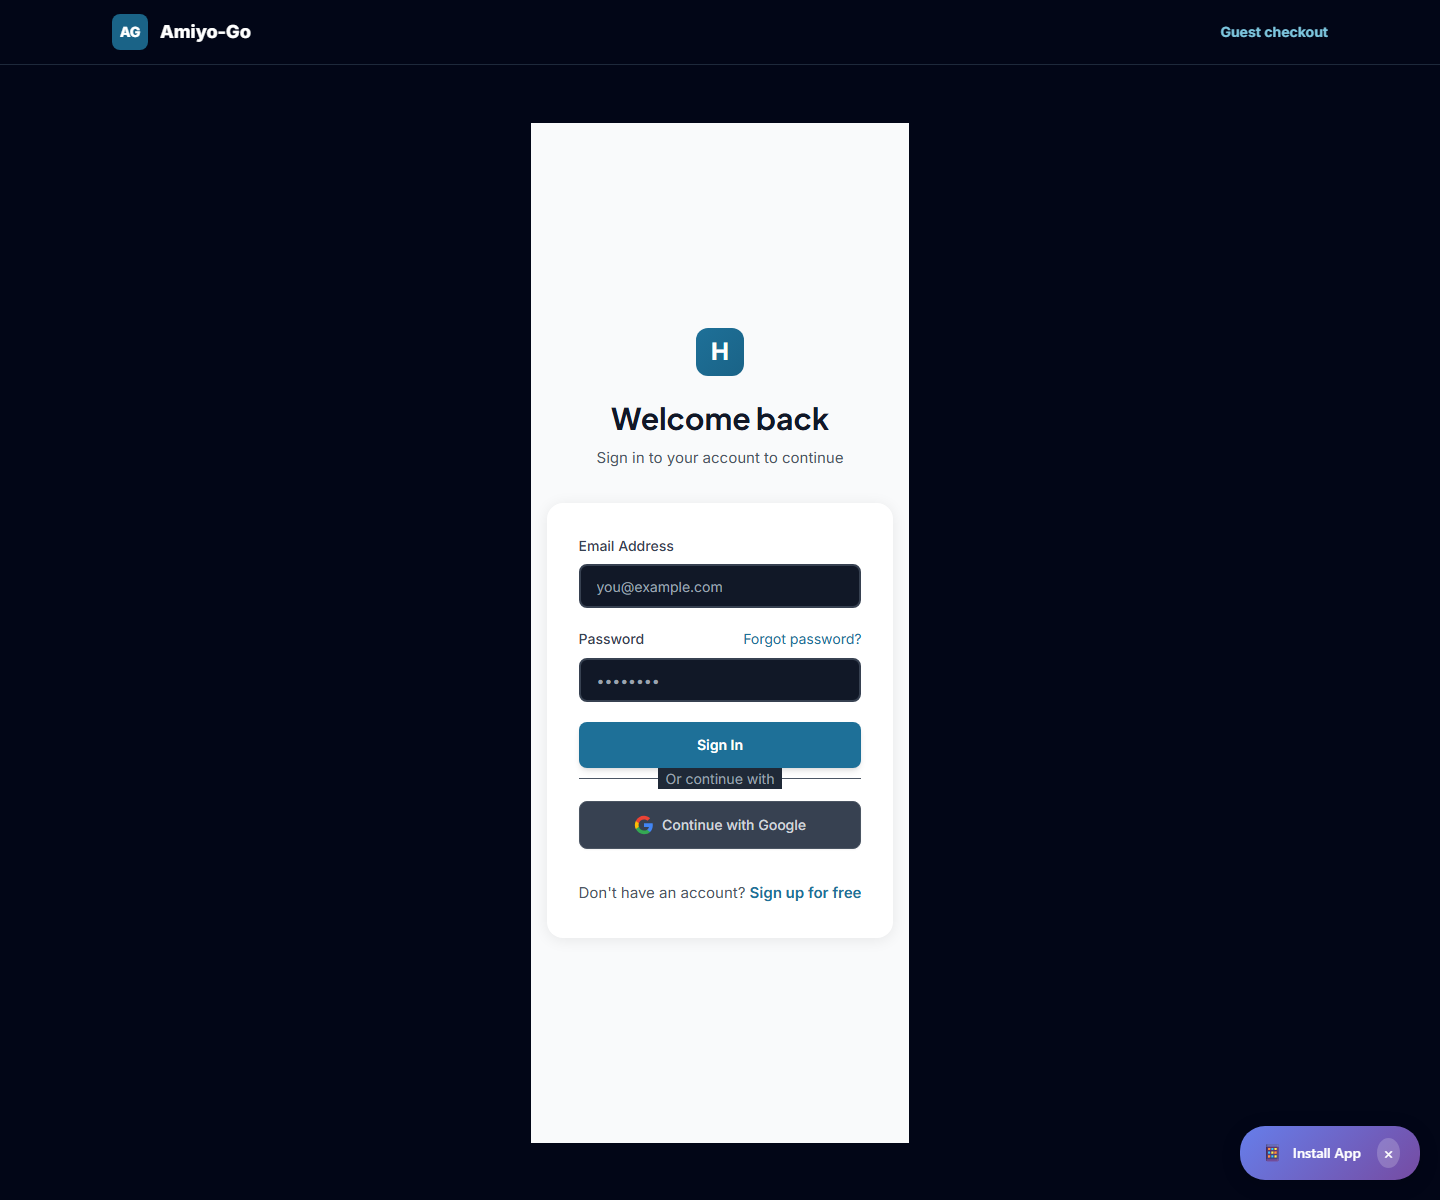
\includegraphics[width=\linewidth,height=0.58\textheight,keepaspectratio]{docs/thesis-screenshots/05-login-access.png}
\caption{Login page for customer, vendor, and admin access}
\end{figure}


\textbf{How it works in English:}


\begin{itemize}
\item Users sign in before accessing protected customer, vendor, or admin pages.
\item Route guards redirect unauthenticated users to login.
\item Admin and vendor pages also check role/permission after authentication.
\item Guest checkout remains available where the project allows it.
\end{itemize}

\textbf{কীভাবে কাজ করে বাংলায়:}


\begin{itemize}
\item Protected customer, vendor বা admin page access করার আগে user sign in করে।
\item Route guard unauthenticated user-কে login page-এ পাঠায়।
\item Admin এবং vendor page authentication-এর পরে role/permission check করে।
\item Project যেখানে allow করে সেখানে guest checkout available থাকে।
\end{itemize}

\subsection{Figure 6: Mobile Home Experience}

\begin{figure}[htbp]
\centering
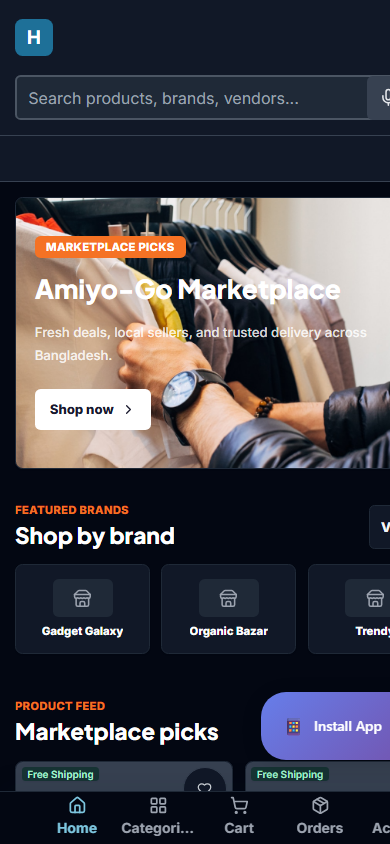
\includegraphics[width=\linewidth,height=0.58\textheight,keepaspectratio]{docs/thesis-screenshots/06-home-mobile.png}
\caption{Responsive mobile home page}
\end{figure}


\textbf{How it works in English:}


\begin{itemize}
\item The same marketplace experience adapts to a mobile viewport.
\item Navigation, category discovery, cart, and account access remain reachable.
\item PWA support allows the site to behave closer to an installable app.
\item Mobile layout is important because marketplace traffic is usually phone-heavy.
\end{itemize}

\textbf{কীভাবে কাজ করে বাংলায়:}


\begin{itemize}
\item একই marketplace experience mobile viewport অনুযায়ী responsive হয়।
\item Navigation, category discovery, cart এবং account access সহজে পাওয়া যায়।
\item PWA support site-কে installable app-এর মতো ব্যবহারযোগ্য করে।
\item Marketplace traffic সাধারণত mobile-heavy হওয়ায় mobile layout খুব গুরুত্বপূর্ণ।
\end{itemize}

\begin{CodeBlock}
---
\end{CodeBlock}

\chapter{Chapter 6: Frontend Architecture}

\section{6.1 Public and Customer Pages}

Important customer-facing pages include:


\begin{itemize}
\item Home.
\item Products.
\item Product detail.
\item Category page.
\item Search results.
\item Shops listing.
\item Shop detail.
\item Cart.
\item Checkout and guest checkout.
\item Order confirmation.
\item Orders.
\item Order detail.
\item Returns.
\item Wishlist.
\item Compare.
\item Loyalty dashboard.
\item Notifications.
\item Messages/support.
\item My reviews.
\item Profile and addresses.
\item Flash sales.
\item Campaign landing.
\item University customer learning page.
\end{itemize}

\section{6.2 Vendor Pages}

Important vendor pages include:


\begin{itemize}
\item Vendor dashboard.
\item Vendor KYC.
\item Vendor shop settings.
\item Vendor shop profile.
\item Vendor bank settings.
\item Vendor category requests.
\item Vendor products.
\item Add/edit product.
\item Bulk upload.
\item Product detail.
\item Orders and order detail.
\item Returns and return detail.
\item Finance.
\item Marketing.
\item Reports.
\item Reviews.
\item Q\&A.
\item Messages/support chat.
\item Protected Vendor University.
\end{itemize}

\section{6.3 Admin Pages}

Important admin pages include:


\begin{itemize}
\item Admin dashboard.
\item Operations center.
\item Vendors and vendor KYC.
\item Vendor chats.
\item Products and product moderation.
\item Category management.
\item Dynamic categories.
\item Category requests.
\item Orders.
\item Returns.
\item Payment verifications.
\item Finance and payouts.
\item COD delivery/reconciliation.
\item Logistics.
\item Delivery settings.
\item Promotions, offers, coupons, vouchers, flash sales.
\item Banners and home controls.
\item Newsletter.
\item Customers and customer insights.
\item Reviews and Q\&A moderation.
\item Support.
\item Trust and safety.
\item User/staff management.
\item Platform controls/settings.
\item Audit logs.
\item Analytics reports.
\item Protected Admin University.
\end{itemize}

\section{6.4 UI and Styling Pattern}

The frontend uses Tailwind CSS with reusable components. UI patterns include:


\begin{itemize}
\item Cards for repeated items.
\item Data tables for admin and vendor queues.
\item Status badges for workflow states.
\item Filter bars and saved views.
\item Mobile bottom navigation.
\item Professional home page sections.
\item Product cards with badges and vendor links.
\item Shop storefront headers, tabs, maps, and product grids.
\item Dashboard metric cards and queue cards.
\end{itemize}

\section{6.5 State and Data Access Pattern}

The project primarily uses React state, context-style utilities, axios/fetch API calls, and route-level data loading patterns. Authentication state is integrated with Firebase and role guards. Some pages use local state and effect-driven fetching, while service modules centralize API calls in several domains.


\begin{CodeBlock}
---
\end{CodeBlock}

\chapter{Chapter 7: Backend Architecture}

\section{7.1 API Layer}

The backend API is organized through Express route modules under \texttt{Server/routes}. \texttt{Server/index.js} registers the domain routes and applies middleware such as:


\begin{itemize}
\item Helmet security headers.
\item CORS configuration.
\item JSON body limits.
\item Request sanitization.
\item Rate limits for API, search, uploads, product views, and payments.
\item Static upload serving.
\item Audit middleware for sensitive actions.
\item Error handling.
\end{itemize}

\section{7.2 Service Layer}

Service modules under \texttt{Server/services} handle reusable business logic. Important services include:


\begin{itemize}
\item Marketplace event bus.
\item Order event service.
\item Notification services.
\item Email and push services.
\item Invoice generation.
\item Promotion service.
\item Promotion rules engine.
\item Discount calculator service.
\item Loyalty service.
\item Recommendation service.
\item Growth event bus and growth notification service.
\item Analytics event and warehouse services.
\item Trust policy, risk scoring, trust case, and enforcement services.
\item Courier provider service.
\item Amiyo Delivery integration service.
\item Payment provider services.
\item Search provider registry and Mongo search provider.
\item Upload and storage services.
\item Bulk upload queue.
\end{itemize}

\section{7.3 Utility Layer}

Utilities support cross-cutting logic:


\begin{itemize}
\item Logistics state machine.
\item Logistics scope helpers.
\item Delivery calculator.
\item Customer order experience.
\item Manual payment proof helpers.
\item Vendor settlement.
\item Vendor staff audit.
\item Platform features.
\item Geocoding with Nominatim.
\item Query optimizer.
\end{itemize}

\section{7.4 Model Layer}

The backend model layer uses Mongoose schemas for major collections:


\begin{itemize}
\item User.
\item Vendor.
\item VendorStaff.
\item VendorShop.
\item Product.
\item Category.
\item DynamicProduct.
\item DynamicCategory.
\item Order.
\item VendorOrder.
\item Shipment.
\item Return.
\item Payment.
\item PaymentVerification.
\item Coupon.
\item Offer.
\item Promotion.
\item Campaign.
\item FlashSale.
\item Review.
\item Question.
\item SupportTicket.
\item Notification.
\item Loyalty.
\item Wishlist.
\item StockAlert.
\item VendorPayout.
\item TrustSafety.
\item AuditLog.
\item AnalyticsSummary.
\item Banner.
\item DeliverySettings.
\item StoreLocation.
\end{itemize}

\begin{CodeBlock}
---
\end{CodeBlock}

\chapter{Chapter 8: Database and Persistence Model}

\section{8.1 Current Database}

The current data store is MongoDB. The project uses both Mongoose models and native MongoDB access in places. This is important because some target architecture diagrams may mention PostgreSQL as a future migration target, but the current implementation is MongoDB.


\section{8.2 Core Persistence Groups}

\begin{CodeBlock}
| Domain | Main models/collections |
\end{CodeBlock}
\begin{CodeBlock}
| --- | --- |
\end{CodeBlock}
\begin{CodeBlock}
| Identity | User, Firebase identity claims, staff permissions |
\end{CodeBlock}
\begin{CodeBlock}
| Vendor | Vendor, VendorShop, VendorStaff, VendorKYC fields |
\end{CodeBlock}
\begin{CodeBlock}
| Catalog | Product, Category, DynamicCategory, DynamicProduct |
\end{CodeBlock}
\begin{CodeBlock}
| Cart/Wishlist | Frontend cart state, Wishlist, StockAlert |
\end{CodeBlock}
\begin{CodeBlock}
| Checkout/Orders | Order, VendorOrder, OrderEvent |
\end{CodeBlock}
\begin{CodeBlock}
| Payments | Payment, PaymentVerification, provider transaction fields |
\end{CodeBlock}
\begin{CodeBlock}
| Logistics | Shipment, delivery settings, dispatch assignments, courier metadata |
\end{CodeBlock}
\begin{CodeBlock}
| Returns | Return, reverse logistics fields, refund state |
\end{CodeBlock}
\begin{CodeBlock}
| Reviews/Q&A | Review, Question |
\end{CodeBlock}
\begin{CodeBlock}
| Support | SupportTicket, LiveChat, VendorChat, AdminVendorChat |
\end{CodeBlock}
\begin{CodeBlock}
| Promotions | Coupon, Voucher routes, Offer, Promotion, Campaign, FlashSale |
\end{CodeBlock}
\begin{CodeBlock}
| Loyalty | Loyalty wallet/transactions and rewards |
\end{CodeBlock}
\begin{CodeBlock}
| Notifications | Notification, NotificationSubscription, PushSubscription |
\end{CodeBlock}
\begin{CodeBlock}
| Trust | TrustSafety, risk events, reports, disputes, enforcements, appeals patterns |
\end{CodeBlock}
\begin{CodeBlock}
| Analytics | AnalyticsSummary, event stream services, campaign analytics |
\end{CodeBlock}
\begin{CodeBlock}
| Admin/Audit | AuditLog, Permission, platform settings |
\end{CodeBlock}

\section{8.3 Data Principles}

The project follows these data principles:


\begin{itemize}
\item Store order snapshots for price, discount, delivery fee, and promotion logic.
\item Split master orders into vendor orders for seller-center workflows.
\item Preserve payment and manual verification state separately from order display.
\item Keep shipment state machine fields separate from reverse logistics and COD state.
\item Use audit logs for sensitive admin actions.
\item Store promotion snapshots so historical orders remain accurate after rules change.
\item Separate public shop data from sensitive vendor KYC/bank data.
\end{itemize}

\begin{CodeBlock}
---
\end{CodeBlock}

\chapter{Chapter 9: Feature Documentation by Role}

\section{9.1 Customer Features}

\subsection{9.1.1 Account and Identity}

Customers can:


\begin{itemize}
\item Register and login.
\item Logout.
\item Reset password.
\item Manage profile.
\item Use guest checkout where enabled.
\item Manage saved addresses.
\item Set default delivery address.
\item Configure notification preferences.
\item Request account export/delete through account routes.
\end{itemize}

\subsection{9.1.2 Discovery and Shopping}

Customers can:


\begin{itemize}
\item Browse home page sections.
\item Browse categories.
\item Search products.
\item Use filters and sorting.
\item View product detail.
\item View vendor storefronts.
\item Browse all shops.
\item Follow shops.
\item Use wishlist.
\item Compare products.
\item View recently viewed and recommendation surfaces.
\item Access flash sales and campaign pages.
\end{itemize}

\subsection{9.1.3 Product Detail}

Product detail supports:


\begin{itemize}
\item Media gallery.
\item Variant selection.
\item Product video support where media URL exists.
\item Badges and trust signals.
\item Delivery estimate widget.
\item Product Q\&A.
\item Reviews with rich review components.
\item Seller info strip.
\item Share/report actions.
\item Frequently bought together.
\item Product recommendations.
\item Stock alert button.
\end{itemize}

\subsection{9.1.4 Cart and Checkout}

Checkout supports:


\begin{itemize}
\item Cart item management.
\item Vendor-grouped cart behavior where implemented.
\item Coupon/voucher validation.
\item Loyalty points redemption.
\item Shipping/delivery fee display.
\item Address selection.
\item Payment method selection.
\item COD and manual/online payment patterns.
\item Guest checkout.
\item Discount persistence into order, invoice, and order detail.
\end{itemize}

\subsection{9.1.5 Orders and Post-Purchase}

Customers can:


\begin{itemize}
\item View order history.
\item Open order detail.
\item Track shipment.
\item See courier assignment when available.
\item See item subtotal, delivery charge, discount, and final total.
\item Reorder.
\item Download or view invoice where enabled.
\item Request return/refund.
\item Review purchased products.
\item Open support.
\end{itemize}

\subsection{9.1.6 Engagement}

Customer engagement includes:


\begin{itemize}
\item Notifications.
\item Push subscriptions.
\item Wishlist alerts.
\item Stock alerts.
\item Loyalty dashboard.
\item Rewards.
\item Followed vendor signals.
\item Amiyo-Go University customer guide.
\end{itemize}

\section{9.2 Vendor Features}

\subsection{9.2.1 Onboarding}

Vendors can:


\begin{itemize}
\item Register as seller.
\item Submit KYC.
\item Manage shop profile.
\item Add pickup/contact information.
\item Request category access.
\item See vendor status.
\item Use protected vendor dashboard after approval.
\end{itemize}

\subsection{9.2.2 Shop Management}

Vendor shop tools include:


\begin{itemize}
\item Shop settings.
\item Shop media.
\item Shop location.
\item Public storefront data.
\item Slug-based shop URLs.
\item Banner/logo.
\item Tagline and description.
\item Policies.
\item Working hours.
\item Social links.
\item Vendor categories.
\end{itemize}

\subsection{9.2.3 Product and Inventory}

Vendors can:


\begin{itemize}
\item Add products.
\item Edit products.
\item Save product fields and variants.
\item Upload product images.
\item Submit for moderation.
\item View rejected/pending/approved states.
\item Use bulk upload jobs.
\item Track product detail and product performance.
\item Handle stock and low stock workflows.
\end{itemize}

\subsection{9.2.4 Orders and Fulfillment}

Vendors can:


\begin{itemize}
\item View vendor order queues.
\item Open order details.
\item Process orders.
\item Add notes where supported.
\item Pack items.
\item Print packing slips/labels where workflow supports it.
\item Mark pickup-ready.
\item Work with logistics and courier assignment.
\item Handle returns and disputes.
\end{itemize}

\subsection{9.2.5 Finance}

Vendor finance includes:


\begin{itemize}
\item Earnings dashboard.
\item Commission visibility.
\item Refund and deduction visibility.
\item COD settlement visibility.
\item Payout request and history.
\item Bank settings.
\item Finance ledger style views.
\end{itemize}

\subsection{9.2.6 Marketing and Reputation}

Vendors can:


\begin{itemize}
\item Manage marketing/vouchers.
\item Join or participate in campaigns where enabled.
\item Track reports.
\item View reviews.
\item Reply or manage reputation workflows where implemented.
\item Use Q\&A.
\item Use vendor support chat.
\item Learn through protected Vendor University.
\end{itemize}

\section{9.3 Admin Features}

\subsection{9.3.1 Platform Control}

Admins can:


\begin{itemize}
\item Access admin dashboard.
\item Use RBAC-aware admin navigation.
\item Manage staff.
\item Use platform settings.
\item View audit logs.
\item Use admin operations center.
\item Use admin global search.
\item Control home banners and sections.
\end{itemize}

\subsection{9.3.2 Vendor Management}

Admins can:


\begin{itemize}
\item Review vendor applications.
\item Review KYC.
\item Approve/reject/suspend vendors.
\item Review vendor details.
\item Monitor vendor performance.
\item Manage vendor categories.
\item Review vendor staff and access patterns.
\end{itemize}

\subsection{9.3.3 Product and Catalog Operations}

Admins can:


\begin{itemize}
\item View all products.
\item Moderate pending products.
\item Approve/reject/disable products.
\item Bulk moderate products.
\item Scan moderation config.
\item Review duplicates.
\item Review IP/counterfeit reports.
\item Manage categories and dynamic categories.
\item Manage category fields/attributes.
\end{itemize}

\subsection{9.3.4 Orders and Returns}

Admins can:


\begin{itemize}
\item View and search global orders.
\item Export orders.
\item View returns queue.
\item Review return evidence.
\item Approve/reject/escalate returns.
\item Process refund states through finance routes.
\item Monitor delivery failures and logistics exceptions.
\end{itemize}

\subsection{9.3.5 Finance and Payouts}

Admins can:


\begin{itemize}
\item Verify manual payments.
\item Approve/reject payment proof.
\item Use payment verification bulk actions.
\item View finance operations.
\item Manage payout queue.
\item Approve/reject/mark payout paid.
\item Manage commission rules.
\item View refund workflow.
\item Export revenue reports.
\item Reconcile COD.
\item Monitor payout exposure.
\end{itemize}

\subsection{9.3.6 Logistics}

Admins can:


\begin{itemize}
\item View logistics dashboard.
\item View state machine.
\item List shipments.
\item Assign courier.
\item Update shipment state.
\item Record delivery attempts.
\item Mark return-to-origin.
\item Confirm RTO received.
\item Generate labels.
\item Confirm manifest pickup.
\item Download waybill.
\item Manage COD state.
\item Manage delivery zones.
\item Manage courier partners.
\item Manage dispatch manifest.
\item Manage pickup staff.
\item Manage delivery fee rules.
\item Monitor failed deliveries.
\end{itemize}

\subsection{9.3.7 Growth and Promotions}

Admins can:


\begin{itemize}
\item Manage coupons/vouchers.
\item Manage offers.
\item Manage promotions.
\item Pause/resume/expire/duplicate promotions.
\item Manage flash sales.
\item Manage campaigns.
\item Manage banners.
\item Manage notification templates/logs.
\item Run abandoned cart detection.
\item Review growth analytics.
\item Manage experiments where enabled.
\end{itemize}

\subsection{9.3.8 Trust and Safety}

Admins can:


\begin{itemize}
\item Review trust and safety dashboard.
\item Process reports.
\item Review disputes.
\item Apply enforcement actions.
\item Handle appeals patterns.
\item Review suspicious reviews, returns, vendors, payouts, and promotions.
\item Use risk scoring and trust policy services.
\end{itemize}

\subsection{9.3.9 Analytics and Reporting}

Admins can:


\begin{itemize}
\item View analytics reports.
\item Use KPI framework and event services.
\item Review growth analytics.
\item Review customer insights.
\item Export reports.
\item Track logistics, finance, trust, growth, campaign, and operational metrics.
\end{itemize}

\begin{CodeBlock}
---
\end{CodeBlock}

\chapter{Chapter 10: Business Workflows}

\section{10.1 Customer Purchase Workflow}

\begin{CodeBlock}
Customer visits home
-> browses category/search/shop/product
-> opens product detail
-> selects variant
-> adds to cart
-> applies voucher/points if available
-> selects address
-> selects payment method
-> reviews order total
-> places order
-> order is created
-> vendor order split is created
-> payment/COD state is recorded
-> shipment draft or logistics state is prepared
-> customer tracks order
-> customer receives item
-> review/return/support is possible
\end{CodeBlock}

\section{10.2 Discount Persistence Workflow}

\begin{CodeBlock}
Checkout validates coupon or promotion
-> backend recalculates discount on order placement
-> order stores discount breakdown and final total
-> invoice reads stored discounted totals
-> order list/detail displays payable amount
-> vendor/admin views use stored order snapshot
\end{CodeBlock}

This workflow prevents the mismatch where checkout shows a discount but order or invoice shows the original price.


\section{10.3 Vendor Product Workflow}

\begin{CodeBlock}
Vendor creates product
-> saves product information, category, images, price, stock
-> submits product for moderation
-> admin reviews listing
-> approved product becomes public
-> rejected product returns with reason
-> vendor edits and resubmits if needed
\end{CodeBlock}

\section{10.4 Vendor Fulfillment Workflow}

\begin{CodeBlock}
Customer places order
-> vendor receives vendor order
-> vendor verifies item/payment/address
-> vendor packs item
-> vendor marks pickup-ready
-> admin/vendor courier workflow starts
-> shipment moves through logistics state machine
-> delivered, failed, or RTO state is recorded
-> finance settlement follows payment and delivery state
\end{CodeBlock}

\section{10.5 Admin Exception Workflow}

\begin{CodeBlock}
Order/vendor/product/return/payment/logistics issue enters queue
-> admin filters and assigns case
-> admin reviews evidence and linked records
-> admin takes allowed action
-> audit log records action
-> notification or workflow state updates affected roles
\end{CodeBlock}

\section{10.6 Return Workflow}

\begin{CodeBlock}
Customer requests return
-> vendor/admin reviews request and evidence
-> return approved/rejected/escalated
-> reverse logistics is scheduled if approved
-> returned item is received
-> item is inspected
-> restock/dispose/refurbish decision is recorded
-> refund and vendor deduction are applied
\end{CodeBlock}

\section{10.7 COD Workflow}

\begin{CodeBlock}
COD pending
-> courier collects cash at delivery
-> COD collected
-> courier/platform remits cash
-> COD remitted
-> platform settles vendor after deductions
\end{CodeBlock}

Exception states include COD failed and COD disputed.


\section{10.8 Protected University Workflow}

\begin{CodeBlock}
Public user opens /university
-> sees customer-only learning content

Vendor opens /vendor/university
-> route guard protects seller learning content

Admin opens /admin/university
-> admin permission guard protects operator learning content
\end{CodeBlock}

This prevents public users from viewing internal vendor/admin operating guidance.


\section{10.9 End-to-End Operating Narrative in English}

Amiyo-Go works as a connected marketplace loop. The customer starts from the home page, search, categories, or shops. After choosing a product, the customer checks price, stock, seller information, delivery estimate, reviews, Q\&A, and available offers. The customer adds items to cart, applies vouchers or loyalty points, selects an address and payment method, then places the order.


When the order is placed, the backend recalculates totals and stores a final order snapshot. This snapshot includes subtotal, delivery charge, discount, payable total, promotion details, payment method, customer address, and item information. The master order is split into vendor orders so each seller can process only their part of the purchase.


The vendor receives the vendor order in the seller center. The vendor checks item, stock, payment state, and delivery address. The vendor packs the product, prepares slip/label where available, and marks the order pickup-ready. Admin or vendor logistics workflows then assign courier, schedule pickup, update shipment state, and track delivery.


If the order is COD, COD state runs beside shipment state. If delivery succeeds, COD can move from pending to collected, remitted, and settled. If delivery fails, admin can record delivery attempts, re-attempt delivery, or mark return-to-origin. If the customer requests a return after delivery, reverse logistics starts and the item moves through approval, pickup, received, inspection, and final stock/refund decision.


The admin controls the marketplace by queues. Admins review vendor applications, product moderation, payments, returns, payouts, logistics exceptions, COD reconciliation, support tickets, trust cases, campaigns, staff permissions, analytics, and audit logs. This queue-first model keeps customer, vendor, and platform operations connected and traceable.


\section{10.10 সম্পূর্ণ কাজের ধারা বাংলায়}

Amiyo-Go একটি connected marketplace loop হিসেবে কাজ করে। Customer home page, search, category বা shop থেকে shopping শুরু করে। Product বাছাই করার পরে customer price, stock, seller information, delivery estimate, review, Q\&A এবং available offer দেখে। এরপর cart-এ item যোগ করে, voucher বা loyalty point apply করে, address ও payment method select করে order place করে।


Order place হলে backend আবার total calculate করে final order snapshot save করে। এই snapshot-এ subtotal, delivery charge, discount, payable total, promotion details, payment method, customer address এবং item information থাকে। Master order vendor order-এ split হয়, যাতে প্রতিটি seller শুধু তার নিজের order অংশ process করতে পারে।


Vendor seller center-এ vendor order পায়। Vendor item, stock, payment state এবং delivery address check করে। এরপর product pack করে, slip/label ready করে এবং order pickup-ready mark করে। তারপর admin বা vendor logistics workflow courier assign করে, pickup schedule করে, shipment state update করে এবং delivery track করে।


Order যদি COD হয়, তাহলে shipment state-এর পাশাপাশি COD state চলে। Delivery successful হলে COD pending থেকে collected, remitted এবং settled state-এ যেতে পারে। Delivery failed হলে admin delivery attempt record করে, re-attempt দিতে পারে অথবা return-to-origin mark করতে পারে। Delivery-এর পরে customer return request করলে reverse logistics শুরু হয় এবং item approval, pickup, received, inspection ও final stock/refund decision-এর মধ্য দিয়ে যায়।


Admin marketplace queue-based control করে। Admin vendor application, product moderation, payment verification, return, payout, logistics exception, COD reconciliation, support ticket, trust case, campaign, staff permission, analytics এবং audit log manage করে। এই queue-first model customer, vendor এবং platform operation-কে connected এবং traceable রাখে।


\begin{CodeBlock}
---
\end{CodeBlock}

\chapter{Chapter 11: API and Service Map}

\section{11.1 Public and Customer APIs}

Important API groups:


\begin{itemize}
\item \texttt{/api/products}
\item \texttt{/api/search}
\item \texttt{/api/categories}
\item \texttt{/api/shops}
\item \texttt{/api/orders}
\item \texttt{/api/orders/guest}
\item \texttt{/api/payments}
\item \texttt{/api/shipments}
\item \texttt{/api/returns}
\item \texttt{/api/reviews}
\item \texttt{/api/wishlist}
\item \texttt{/api/addresses}
\item \texttt{/api/coupons}
\item \texttt{/api/vouchers}
\item \texttt{/api/offers}
\item \texttt{/api/flash-sales}
\item \texttt{/api/recommendations}
\item \texttt{/api/notifications}
\item \texttt{/api/support}
\item \texttt{/api/loyalty}
\item \texttt{/api/stock-alerts}
\item \texttt{/api/account}
\end{itemize}

\section{11.2 Vendor APIs}

Important vendor API groups:


\begin{itemize}
\item \texttt{/api/vendors}
\item \texttt{/api/vendor/kyc}
\item \texttt{/api/vendors/staff}
\item \texttt{/api/vendor/shop}
\item \texttt{/api/vendor/products}
\item \texttt{/api/vendors/finance}
\item \texttt{/api/vendors} for vendor order management routes.
\item \texttt{/api/vendor/logistics}
\item \texttt{/api/vendor/growth}
\item \texttt{/api/vendor-chat}
\end{itemize}

\section{11.3 Admin APIs}

Important admin API groups:


\begin{itemize}
\item \texttt{/api/admin/dashboard}
\item \texttt{/api/admin/users}
\item \texttt{/api/admin/vendors}
\item \texttt{/api/admin/vendors/kyc}
\item \texttt{/api/admin/products}
\item \texttt{/api/admin/payment-verification}
\item \texttt{/api/admin/banners}
\item \texttt{/api/admin/settings}
\item \texttt{/api/admin/staff}
\item \texttt{/api/admin/vouchers}
\item \texttt{/api/admin/cod}
\item \texttt{/api/admin/reviews}
\item \texttt{/api/admin/orders}
\item \texttt{/api/admin/vendor-marketing}
\item \texttt{/api/admin/finance}
\item \texttt{/api/admin/payouts}
\item \texttt{/api/admin/alerts}
\item \texttt{/api/admin/search}
\item \texttt{/api/admin/promotions}
\item \texttt{/api/admin/growth}
\item \texttt{/api/admin/logistics}
\item \texttt{/api/admin/customers}
\item \texttt{/api/admin/trust-safety}
\item \texttt{/api/admin/platform}
\item \texttt{/api/admin/audit}
\item \texttt{/api/admin/analytics}
\item \texttt{/api/admin/dispatch}
\end{itemize}

\section{11.4 Integration APIs and Services}

Integration-related modules include:


\begin{itemize}
\item Payment provider services.
\item Webhook routes.
\item Courier provider service.
\item Amiyo Delivery integration service.
\item Upload service routes.
\item Email queue and email service.
\item Push service.
\item SMS service placeholder.
\item Analytics event ingestion.
\item Marketplace event bus.
\end{itemize}

\begin{CodeBlock}
---
\end{CodeBlock}

\chapter{Chapter 12: Security, Trust, and Permissions}

\section{12.1 Authentication}

Authentication is integrated with Firebase. Backend routes use token verification middleware and role checks such as admin/vendor/customer route protection.


\section{12.2 Authorization}

Authorization patterns include:


\begin{itemize}
\item AdminRoute and VendorRoute frontend guards.
\item Backend \texttt{verifyToken}, \texttt{verifyAdmin}, and role/permission checks.
\item Admin RBAC and permission-aware navigation.
\item Staff permission controls.
\item Protected vendor/admin University content.
\end{itemize}

\section{12.3 API Protection}

API protection includes:


\begin{itemize}
\item Helmet.
\item CORS configuration.
\item Rate limiting.
\item Mongo sanitization.
\item Upload limits.
\item Payment/search/upload-specific rate limits.
\item Audit middleware for sensitive admin operations.
\end{itemize}

\section{12.4 Trust and Safety}

Trust and safety modules support:


\begin{itemize}
\item Risk scoring.
\item Reports.
\item Disputes.
\item Enforcement.
\item Appeals pattern.
\item Review moderation.
\item Return abuse signals.
\item Promo abuse protection.
\item Payout risk controls.
\item Auditability.
\end{itemize}

\section{12.5 Staff Governance}

Admin can add staff/managers and give section-based permissions. The intended production rule is:


\begin{itemize}
\item Staff can operate assigned sections.
\item Staff should not receive delete/settings permissions unless necessary.
\item Sensitive actions require audit logs.
\item Super-admin-only permissions should remain restricted.
\end{itemize}

\begin{CodeBlock}
---
\end{CodeBlock}

\chapter{Chapter 13: Logistics and Courier Integration}

\section{13.1 Shipment State Machine}

Forward logistics states:


\begin{CodeBlock}
created
-> pending_packing
-> packed
-> pickup_ready
-> pickup_scheduled
-> picked_up
-> in_transit
-> out_for_delivery
-> delivered
\end{CodeBlock}

Exception states:


\begin{CodeBlock}
delivery_failed
-> out_for_delivery
or
delivery_failed
-> return_to_origin
\end{CodeBlock}

\section{13.2 Reverse Logistics State Machine}

\begin{CodeBlock}
return_requested
-> return_approved
-> return_pickup_scheduled
-> return_picked_up
-> return_in_transit
-> return_received
-> inspected
-> restocked / disposed / refurbished
\end{CodeBlock}

\section{13.3 COD State Machine}

\begin{CodeBlock}
cod_pending
-> cod_collected
-> cod_remitted
-> cod_settled
\end{CodeBlock}

Exception states:


\begin{CodeBlock}
cod_failed
cod_disputed
\end{CodeBlock}

\section{13.4 Courier Assignment}

Courier assignment can be:


\begin{itemize}
\item Internal/manual courier.
\item Area-based courier rules.
\item RedX adapter-backed booking when credentials are configured.
\item Steadfast adapter-backed booking when credentials are configured.
\item Amiyo Delivery integration.
\item Future local instant delivery provider.
\end{itemize}

\section{13.5 No-Paid-API Operating Mode}

The marketplace can operate without paid courier APIs by using:


\begin{itemize}
\item Manual courier assignment.
\item Internal courier state updates.
\item Packing and pickup-ready workflow.
\item Manual tracking number entry.
\item Admin logistics dashboard.
\item COD state updates.
\item Manual delivery attempt/RTO handling.
\end{itemize}

This is important because the system can run before every delivery partner is integrated.


\begin{CodeBlock}
---
\end{CodeBlock}

\chapter{Chapter 14: Promotions, Growth, and Personalization}

\section{14.1 Promotion Engine}

Promotion-related features include:


\begin{itemize}
\item Coupons.
\item Vouchers.
\item Offers.
\item Platform promotions.
\item Vendor marketing items.
\item Flash sales.
\item Campaigns.
\item Promotion snapshots.
\item Discount calculators.
\item Stacking/conflict logic patterns.
\end{itemize}

\section{14.2 Loyalty}

Loyalty features include:


\begin{itemize}
\item Loyalty dashboard.
\item Points redemption.
\item Rewards.
\item Customer loyalty ledger patterns.
\item Admin loyalty adjustment.
\end{itemize}

\section{14.3 Recommendations and Discovery}

Discovery and recommendation features include:


\begin{itemize}
\item Product recommendations.
\item Frequently bought together.
\item Similar products.
\item Recently viewed patterns.
\item Search suggestions/history.
\item Shop discovery.
\item Followed vendor signals where enabled.
\end{itemize}

\section{14.4 Notifications}

Notification features include:


\begin{itemize}
\item In-app notification center.
\item Push subscriptions.
\item Email services.
\item Growth notifications.
\item Notification templates/logs in admin growth routes.
\item Order/return/support/promotion notifications where emitted.
\end{itemize}

\begin{CodeBlock}
---
\end{CodeBlock}

\chapter{Chapter 15: Analytics and Reporting}

\section{15.1 Analytics Foundation}

The project includes:


\begin{itemize}
\item Analytics event service.
\item Analytics KPI framework.
\item Analytics warehouse service.
\item Analytics intelligence service.
\item Growth event service.
\item Campaign analytics service.
\item Admin analytics routes.
\item Vendor reports.
\end{itemize}

\section{15.2 KPI Categories}

Customer KPIs:


\begin{itemize}
\item Sessions.
\item Product views.
\item Add-to-cart rate.
\item Checkout rate.
\item Conversion rate.
\item AOV.
\item Repeat purchases.
\item Notification engagement.
\end{itemize}

Vendor KPIs:


\begin{itemize}
\item GMV.
\item Net sales.
\item Order count.
\item Fulfillment speed.
\item Return rate.
\item Cancellation rate.
\item Stockout risk.
\item Review score.
\item Campaign GMV.
\end{itemize}

Admin KPIs:


\begin{itemize}
\item Total GMV.
\item Commission revenue.
\item Refund rate.
\item Payout exposure.
\item COD exposure.
\item RTO rate.
\item Support SLA.
\item Logistics SLA.
\item Fraud/dispute rate.
\item Active customers/vendors.
\end{itemize}

\section{15.3 Report Surfaces}

Report surfaces include:


\begin{itemize}
\item Admin analytics reports.
\item Admin dashboard overview.
\item Admin operations overview.
\item Finance reports and export.
\item Vendor reports.
\item Growth analytics.
\item Campaign analytics.
\item Customer insights.
\item Logistics dashboard.
\item Trust and safety dashboard.
\end{itemize}

\begin{CodeBlock}
---
\end{CodeBlock}

\chapter{Chapter 16: Testing and Quality Assurance}

\section{16.1 Existing Test Structure}

The project contains frontend and backend test scripts:


\begin{itemize}
\item Client: \texttt{npm run test}
\item Client: \texttt{npm run build}
\item Server: \texttt{npm test}
\item Server: \texttt{npm run test:all}
\item Server: API and notification test scripts.
\end{itemize}

Frontend tests exist in areas such as:


\begin{itemize}
\item Route guards.
\item Design system.
\item Delivery estimate widget.
\item Admin dashboard hardening.
\item Vendor home command center.
\end{itemize}

Backend test scripts include:


\begin{itemize}
\item Server health/API tests.
\item Push notification tests.
\item Email checks.
\item Flash sale checks.
\item Performance test script.
\end{itemize}

\section{16.2 Quality Checks Used for This Documentation}

For this documentation package:


\begin{itemize}
\item Existing source files and route maps were inspected.
\item Current feature docs were consolidated.
\item Current backend route registration was reviewed.
\item Frontend page/layout structure was reviewed.
\item PDF generation was implemented with a reusable script.
\end{itemize}

\section{16.3 Recommended Production Test Plan}

Before production release, run:


\begin{enumerate}
\item Client build.
\item Client unit/component tests.
\item Server unit/API tests.
\item Authentication guard tests.
\item Checkout discount persistence test.
\item Order creation and vendor split test.
\item Payment verification workflow test.
\item Courier assignment workflow test.
\item Return/refund/vendor deduction test.
\item Admin RBAC and staff permission test.
\item Shop storefront/follow test.
\item Notification event test.
\item Analytics emission test.
\item Mobile responsive smoke test.
\end{enumerate}

\begin{CodeBlock}
---
\end{CodeBlock}

\chapter{Chapter 17: Deployment and Environment Configuration}

\section{17.1 Client Deployment}

The client is a Vite React app and can be deployed to providers such as Netlify, Vercel, or static hosting. It uses environment variables for API base URL and frontend configuration.


\section{17.2 Server Deployment}

The server is a Node.js Express application. Deployment requires:


\begin{itemize}
\item Node.js runtime.
\item MongoDB connection.
\item Firebase Admin configuration.
\item CORS allowed origins.
\item Upload/storage configuration.
\item Optional Redis.
\item Optional email/push credentials.
\item Optional payment/courier credentials.
\end{itemize}

\section{17.3 Environment Safety}

Never publish real secrets in documentation, screenshots, or public repositories. Use \texttt{.env.example} only for variable names and placeholder values.


Important environment groups:


\begin{itemize}
\item MongoDB URL.
\item Firebase service credentials.
\item JWT/API secrets.
\item CORS origins.
\item Client/server URLs.
\item Courier provider tokens.
\item Payment provider keys.
\item Email credentials.
\item Push VAPID keys.
\item Storage provider credentials.
\item Redis URL.
\end{itemize}

\section{17.4 Operational Dependencies}

The marketplace can run with partial integrations, but production reliability improves when these are configured:


\begin{itemize}
\item Stable MongoDB.
\item Redis for queues.
\item Email provider.
\item Push keys.
\item Payment webhook verification.
\item Courier provider credentials.
\item Storage/CDN provider.
\item Error logging and monitoring.
\end{itemize}

\begin{CodeBlock}
---
\end{CodeBlock}

\chapter{Chapter 18: Documentation and Training Layer}

\section{18.1 Existing Documentation Files}

The repository includes documentation such as:


\begin{itemize}
\item \texttt{README.md}
\item \texttt{README\_ADMIN.md}
\item \texttt{README\_VENDOR.md}
\item \texttt{README\_USER.md}
\item \texttt{ROLE\_FEATURES\_DOCUMENTATION.md}
\item \texttt{MARKETPLACE\_WORKFLOW\_DIAGRAMS.md}
\item \texttt{MARKETPLACE\_ROLE\_WORKFLOWS.md}
\item \texttt{DARAZ\_LEVEL\_MARKETPLACE\_AUDIT.md}
\item \texttt{DARAZ\_PROFESSIONAL\_FEATURE\_GAP\_STATUS.md}
\item \texttt{TESTING\_DOCUMENTATION.md}
\item \texttt{COURIER\_INTEGRATION\_WORKFLOW.md}
\item Dynamic category/product docs.
\end{itemize}

\section{18.2 Amiyo-Go University}

Amiyo-Go University provides role learning:


\begin{itemize}
\item Public \texttt{/university}: customer-only learning content.
\item Protected \texttt{/vendor/university}: vendor learning content.
\item Protected \texttt{/admin/university}: admin/operator learning content.
\end{itemize}

This protects internal operating information from public users while still giving each role contextual guidance.


\begin{CodeBlock}
---
\end{CodeBlock}

\chapter{Chapter 19: Production-Readiness Assessment}

\section{19.1 Strong Areas}

Current strong areas:


\begin{itemize}
\item Role-based marketplace architecture.
\item Large admin control surface.
\item Vendor seller-center pages.
\item Customer shopping and post-purchase flows.
\item Shop storefront feature.
\item Discount persistence improvements.
\item Logistics state machine foundations.
\item COD and reverse logistics state foundations.
\item Promotion, flash sale, loyalty, and growth foundations.
\item Trust and safety foundations.
\item Analytics/reporting foundations.
\item Staff/RBAC patterns.
\item Documentation and training layer.
\end{itemize}

\section{19.2 Remaining Hardening Areas}

High-value production hardening still recommended:


\begin{itemize}
\item Make BullMQ event bus universal for all order/payment/return/support/logistics events.
\item Expand failed-job and failed-notification monitoring UI.
\item Strengthen end-to-end tests for every admin queue.
\item Add more complete payment provider webhook coverage.
\item Add real courier API production booking and tracking after provider selection.
\item Improve analytics emission audit for every state transition.
\item Add more observability for queue lag, stale dashboards, and failed integrations.
\item Add stricter secret scanning and environment validation.
\item Add formal release checklist and rollback procedure.
\end{itemize}

\section{19.3 Market Launch Readiness}

Amiyo-Go has enough functional breadth to operate a controlled marketplace pilot if:


\begin{itemize}
\item MongoDB is stable.
\item Auth and CORS are correctly configured.
\item Manual payment verification is operational.
\item Manual/internal courier workflow is accepted initially.
\item Admin staff permissions are configured carefully.
\item Vendors are onboarded with real KYC review.
\item Support and returns policies are clearly published.
\item Operational staff follow queue-based procedures.
\end{itemize}

For high-scale public launch, the hardening areas in section 19.2 should be prioritized.


\begin{CodeBlock}
---
\end{CodeBlock}

\chapter{Chapter 20: Limitations and Future Work}

\section{20.1 Current Limitations}

Known limitations include:


\begin{itemize}
\item Some integrations are adapter-ready but not fully live without credentials.
\item Redis/BullMQ is not yet universal across every workflow.
\item Some analytics dashboards depend on consistent event emission.
\item Some advanced Daraz-level features are present as foundations but need deeper automation.
\item External courier tracking depends on provider API support.
\item Payment gateway behavior depends on provider setup and webhook reliability.
\item Some queue and dashboard views require production data to validate deeply.
\end{itemize}

\section{20.2 Future Work}

Future work should include:


\begin{itemize}
\item Full event bus coverage.
\item Production courier adapters.
\item Payment gateway webhook hardening.
\item Server-side cart persistence with guest merge.
\item Advanced sponsored product advertising.
\item Map-pin address improvements.
\item Deep seller health score automation.
\item More formal fraud thresholds.
\item Scheduled reports and data quality alerts.
\item A/B testing analytics.
\item More comprehensive Playwright/Cypress end-to-end tests.
\item Production monitoring dashboards.
\item Automated backup and restore plan.
\end{itemize}

\begin{CodeBlock}
---
\end{CodeBlock}

\chapter{Chapter 21: Conclusion}

Amiyo-Go is structured as a real marketplace operating system rather than a basic ecommerce app. It supports customer shopping, seller-center operations, and admin governance through role-specific pages, backend domain modules, data models, and workflows.


The current implementation includes strong foundations for catalog, search, checkout, orders, vendor operations, admin operations, logistics, COD, returns, payments, promotions, loyalty, notifications, trust, analytics, staff permissions, shop storefronts, and documentation. The system can operate without paid courier APIs by using manual/internal logistics workflows and can later attach provider APIs through adapter services.


The next stage should focus on reliability, observability, end-to-end testing, queue unification, payment/courier production hardening, and data quality. With those improvements, Amiyo-Go can move closer to a production-grade Daraz-level marketplace.


\begin{CodeBlock}
---
\end{CodeBlock}

\chapter{Appendices}

\section{Appendix A: Feature Matrix}

\begin{CodeBlock}
| Feature Area | Customer | Vendor | Admin |
\end{CodeBlock}
\begin{CodeBlock}
| --- | --- | --- | --- |
\end{CodeBlock}
\begin{CodeBlock}
| Account/profile | Yes | Yes | Staff/admin |
\end{CodeBlock}
\begin{CodeBlock}
| Saved addresses | Yes | Pickup/shop address | View/manage where needed |
\end{CodeBlock}
\begin{CodeBlock}
| Product browse | Yes | Own product view | All products |
\end{CodeBlock}
\begin{CodeBlock}
| Product creation | No | Yes | Admin edit/moderate |
\end{CodeBlock}
\begin{CodeBlock}
| Product moderation | No | Submission/rejection view | Yes |
\end{CodeBlock}
\begin{CodeBlock}
| Shop storefront | Browse/follow | Manage own shop | Control visibility/settings |
\end{CodeBlock}
\begin{CodeBlock}
| Cart/checkout | Yes | No | Order oversight |
\end{CodeBlock}
\begin{CodeBlock}
| Vouchers/promos | Apply | Create/join where enabled | Create/manage |
\end{CodeBlock}
\begin{CodeBlock}
| Orders | Own orders | Vendor orders | Global orders |
\end{CodeBlock}
\begin{CodeBlock}
| Packing/dispatch | Track only | Pack/pickup-ready | Monitor/override |
\end{CodeBlock}
\begin{CodeBlock}
| Courier assignment | View | View/request where enabled | Assign/reassign |
\end{CodeBlock}
\begin{CodeBlock}
| COD | Pay at delivery | Settlement visibility | Reconcile |
\end{CodeBlock}
\begin{CodeBlock}
| Returns | Request | Respond/inspect | Decide/monitor/refund |
\end{CodeBlock}
\begin{CodeBlock}
| Reviews/Q&A | Ask/review | Reply/manage | Moderate |
\end{CodeBlock}
\begin{CodeBlock}
| Support | Create tickets | Vendor messages | Queue/assign/reply |
\end{CodeBlock}
\begin{CodeBlock}
| Finance | Order payment view | Earnings/payouts | Payout/finance controls |
\end{CodeBlock}
\begin{CodeBlock}
| Analytics | Personal surfaces | Vendor reports | Full platform reports |
\end{CodeBlock}
\begin{CodeBlock}
| Trust/safety | Report issues | Respond to cases | Full queue/enforcement |
\end{CodeBlock}
\begin{CodeBlock}
| University | Customer guide | Protected vendor guide | Protected admin guide |
\end{CodeBlock}

\section{Appendix B: Important Commands}

\begin{CodeBlock}
Client:
cd Client
npm run dev
npm run build
npm run test

Server:
cd Server
npm run dev
npm start
npm test
npm run seed
npm run make:admin

Documentation PDF:
node scripts/generateThesisPdf.js
\end{CodeBlock}

\section{Appendix C: Key Route Examples}

\begin{CodeBlock}
Customer:
/products
/product/:id
/shops
/shops/:slug
/cart
/checkout
/orders
/orders/:orderId
/returns
/support
/university

Vendor:
/vendor/dashboard
/vendor/shop/settings
/vendor/products
/vendor/orders
/vendor/finance
/vendor/marketing
/vendor/reports
/vendor/university

Admin:
/admin
/admin/operations
/admin/products
/admin/vendors
/admin/orders
/admin/returns
/admin/logistics
/admin/finance
/admin/payouts
/admin/trust-safety
/admin/analytics
/admin/staff
/admin/university
\end{CodeBlock}

\section{Appendix D: Glossary}

\begin{CodeBlock}
| Term | Meaning |
\end{CodeBlock}
\begin{CodeBlock}
| --- | --- |
\end{CodeBlock}
\begin{CodeBlock}
| COD | Cash on delivery |
\end{CodeBlock}
\begin{CodeBlock}
| RTO | Return to origin |
\end{CodeBlock}
\begin{CodeBlock}
| KYC | Know your customer/business verification |
\end{CodeBlock}
\begin{CodeBlock}
| GMV | Gross merchandise value |
\end{CodeBlock}
\begin{CodeBlock}
| SLA | Service level agreement |
\end{CodeBlock}
\begin{CodeBlock}
| RBAC | Role-based access control |
\end{CodeBlock}
\begin{CodeBlock}
| Vendor order | Vendor-specific split of a customer order |
\end{CodeBlock}
\begin{CodeBlock}
| Promotion snapshot | Saved discount rule result for historical order accuracy |
\end{CodeBlock}
\begin{CodeBlock}
| Reverse logistics | Return shipment workflow after delivery |
\end{CodeBlock}
\begin{CodeBlock}
| Queue-first operations | Admin pattern where staff handle exception queues before routine browsing |
\end{CodeBlock}

\section{Appendix E: Source Documentation References}

This thesis documentation consolidates information from the project source code and existing docs:


\begin{itemize}
\item \texttt{README.md}
\item \texttt{README\_ADMIN.md}
\item \texttt{README\_VENDOR.md}
\item \texttt{README\_USER.md}
\item \texttt{ROLE\_FEATURES\_DOCUMENTATION.md}
\item \texttt{MARKETPLACE\_WORKFLOW\_DIAGRAMS.md}
\item \texttt{MARKETPLACE\_ROLE\_WORKFLOWS.md}
\item \texttt{DARAZ\_LEVEL\_MARKETPLACE\_AUDIT.md}
\item \texttt{DARAZ\_PROFESSIONAL\_FEATURE\_GAP\_STATUS.md}
\item \texttt{TESTING\_DOCUMENTATION.md}
\item \texttt{COURIER\_INTEGRATION\_WORKFLOW.md}
\item \texttt{Server/index.js}
\item \texttt{Server/routes}
\item \texttt{Server/models}
\item \texttt{Server/services}
\item \texttt{Client/src/pages}
\item \texttt{Client/src/components}
\item \texttt{Client/src/layouts}
\item \texttt{Client/src/routes}
\end{itemize}

\end{document}
